\subsection{Modélisation et lissage de la zone de sécurité}

Afin de délimiter la zone de sécurité autour de l'engin de chantier de manière optimale, il est impératif de traiter les nuages de points tridimensionnels bruts renvoyés par les capteurs. Ces points, de par l'incertitude des mesures UWB, présentent des irrégularités spatiales importantes (bruit de mesure). Ils doivent donc être normalisés pour former un plan d'exclusion unifié, clair et exploitable par le Hub. 

Ce processus a été scindé en deux étapes mathématiques implémentées en C++ à l'aide de la librairie \texttt{Eigen} : la définition d'un plan moyen par régression orthogonale et le rééchantillonnage géométrique du polygone.

\begin{figure}[!ht]
\centering 
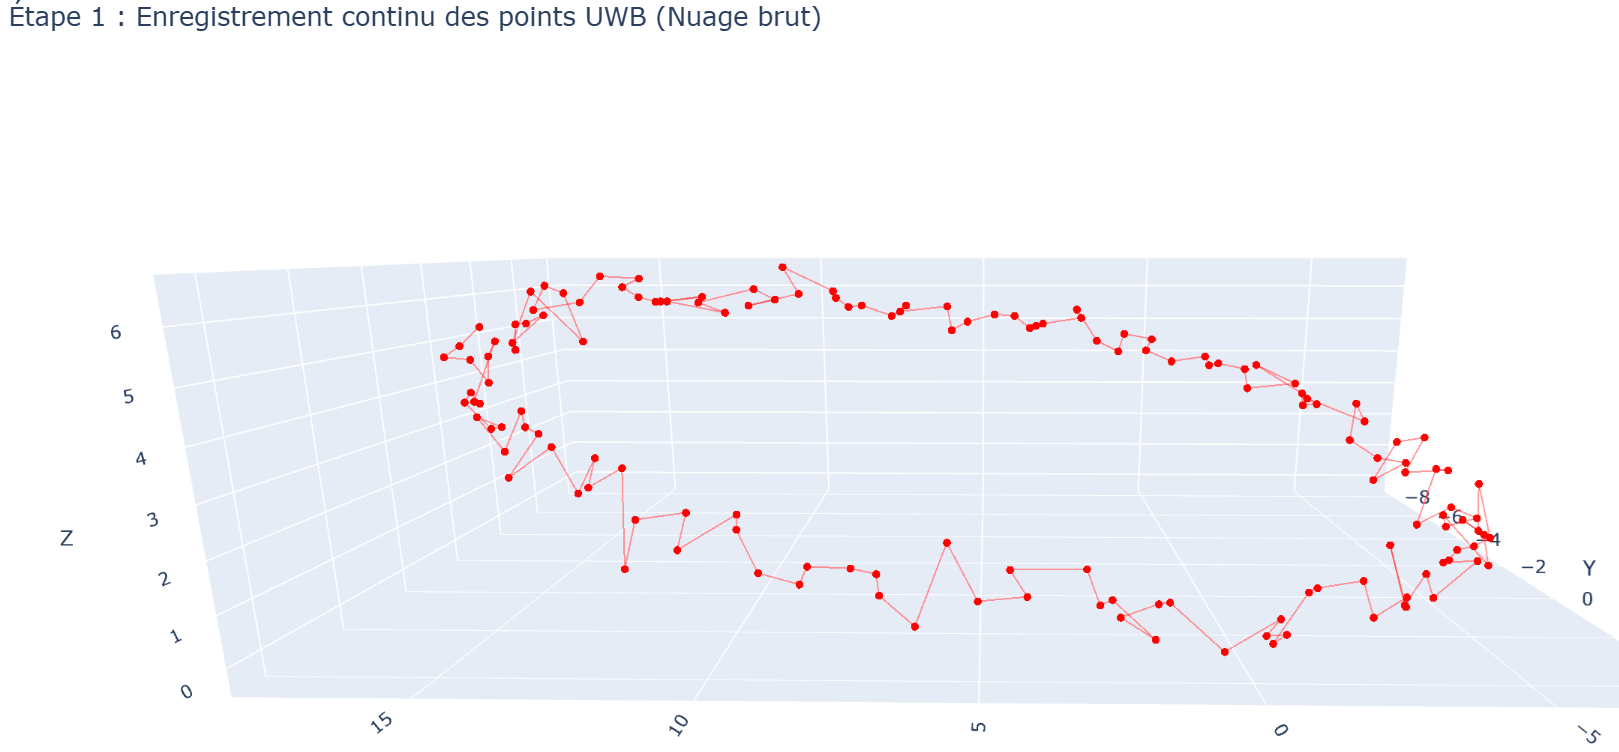
\includegraphics[width=0.6\columnwidth]{Figures/fig1_points_initiaux.png} 
\caption[Points UWB bruts]{Représentation tridimensionnelle d'un nuage de points initial bruité.}
\end{figure}

\subsubsection{Détermination du plan local par ACP}

La première étape, implémentée dans la fonction \texttt{calculerPlanMoyen}, consiste à déterminer le plan se rapprochant le plus de notre ensemble de points tridimensionnels en minimisant la distance orthogonale de chaque point au plan. Pour ce faire, nous appliquons une Analyse en Composantes Principales (ACP).

Dans un premier temps, nous calculons le barycentre des points, qui constituera l'origine spatiale de notre plan local. En notant $n$ le nombre total de points et $P_i$ les coordonnées d'un point donné, le centre de gravité $C$ est défini par :

\begin{equation}
    C = \frac{1}{n} \sum_{i=1}^{n} P_i
\end{equation}

Une fois les points centrés sur ce barycentre, nous calculons leur matrice de covariance empirique. La factorisation de cette matrice nous permet d'extraire ses vecteurs propres. Le vecteur propre associé à la plus petite valeur propre correspond à la direction de variance minimale, et définit donc la normale du plan d'exclusion, notée $\vec{n}$. 

À partir de cette normale et d'un vecteur arbitraire non colinéaire, nous utilisons le produit vectoriel pour générer deux vecteurs orthogonaux unitaires, $\vec{u}$ et $\vec{v}$. Le triplet $(C, \vec{u}, \vec{v})$ constitue la base de notre repère local euclidien en deux dimensions.

\begin{figure}[!ht]
\centering 
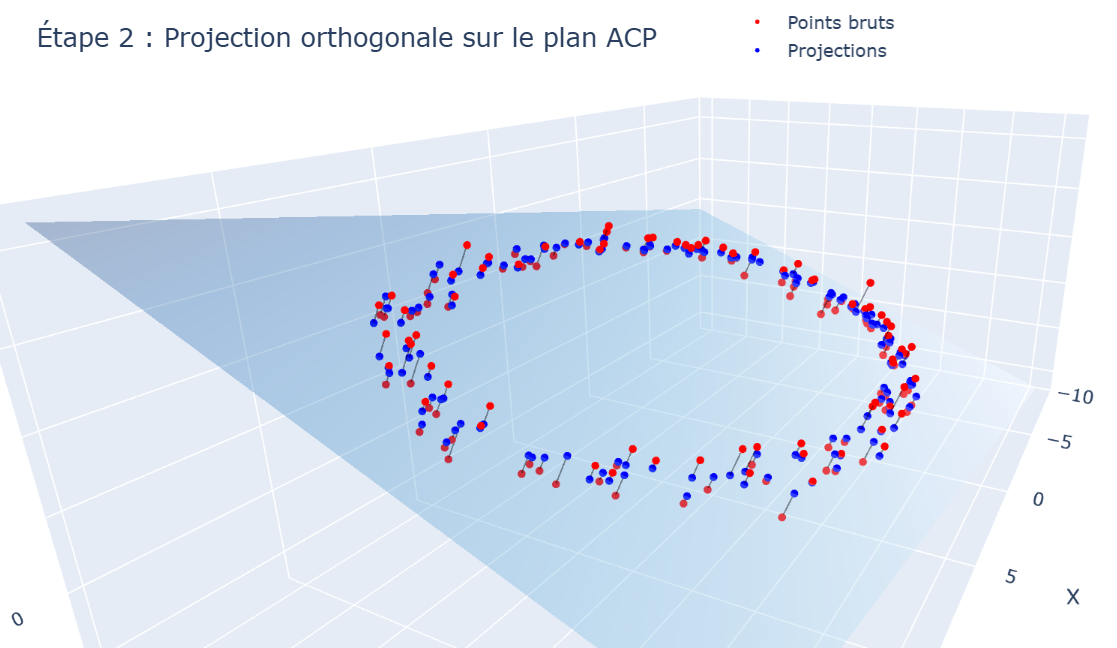
\includegraphics[width=0.6\columnwidth]{Figures/fig2_projection_plan.png} 
\caption[Projection sur plan ACP]{Calcul du plan moyen et projection orthogonale des points sur la base locale $(\vec{u}, \vec{v})$.}
\end{figure}

\subsubsection{Projection 2D et rééchantillonnage régulier}

Une fois le plan mathématique établi, la fonction \texttt{echantillonner64Points} est employée pour uniformiser la géométrie de la zone. Les contraintes matérielles liées à l'utilisation des microcontrôleurs ESP32 nécessitent de travailler avec des structures de données de taille fixe afin de garantir un temps de calcul constant ($\mathcal{O}(1)$ en allocation). 

La taille du polygone a ainsi été fixée à 64 points. Cette valeur n'est pas arbitraire : elle correspond à un compromis optimal offrant une résolution visuelle suffisamment fine pour l'affichage sur l'écran de l'interface utilisateur de l'engin, tout en minimisant la charge mémoire. De plus, sur ces 64 points, l'algorithme ne calcule par interpolation que 63 points intermédiaires. Le point d'indice 0 est le point de départ projeté, et le 64\textsuperscript{ème} point (indice 63) est strictement identique au premier, garantissant ainsi la fermeture parfaite du polygone géométrique.

L'algorithme opère selon le processus suivant :

\begin{itemize}
    \item \textbf{Projection :} Chaque point 3D initial est projeté orthogonalement sur le plan local 2D défini par la base $(\vec{u}, \vec{v})$.
    \item \textbf{Calcul du périmètre :} La distance euclidienne entre chaque sommet projeté est cumulée pour obtenir le périmètre total du polygone brut.
    \item \textbf{Interpolation linéaire :} Le périmètre est divisé par 63 pour définir une longueur de segment constante, appelée "pas d'échantillonnage". L'algorithme parcourt ensuite les arêtes du polygone initial et calcule par interpolation les coordonnées exactes des nouveaux points à chaque pas.
    \item \textbf{Reprojection 3D :} Les nouvelles coordonnées 2D lissées sont multipliées par les vecteurs directeurs $\vec{u}$ et $\vec{v}$, puis additionnées au centre $C$, pour repasser dans le repère virtuel en trois dimensions du Hub.
\end{itemize}

\begin{figure}[H]
\centering 
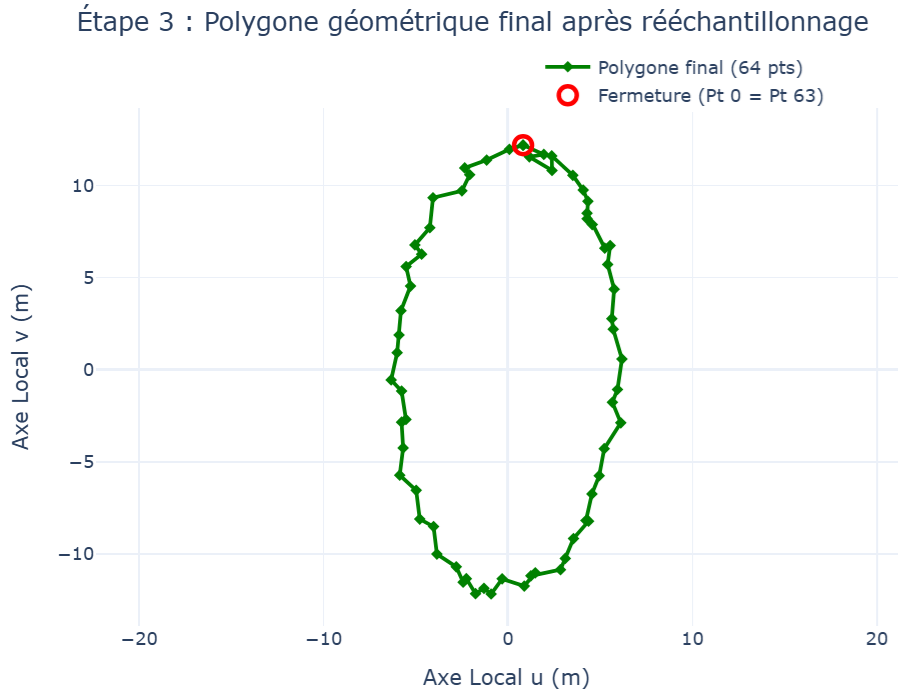
\includegraphics[width=0.6\columnwidth]{Figures/fig3_polygone_lisse.png} 
\caption[Rééchantillonnage du polygone]{Comparaison entre le polygone brut projeté et le polygone final lissé à 64 points équidistants.}
\end{figure}

Cette approche mathématique garantit la création d'un polygone fermé, parfaitement coplanaire, dont la distribution régulière des sommets optimise considérablement les futurs calculs de détection de franchissement de zone par les ouvriers.